\documentclass[10pt,a4paper]{article}
\usepackage[margin=22mm]{geometry}
\usepackage[T1]{fontenc}
\usepackage{lmodern,microtype,amsmath,amssymb,booktabs,graphicx}
\usepackage[colorlinks=true,linkcolor=blue,urlcolor=blue,citecolor=blue]{hyperref}
\usepackage{caption}
\captionsetup{font=small,labelfont=bf}
\setlength{\parindent}{0pt}
\setlength{\parskip}{5pt}
\newcommand{\ConvError}{3.331\times10^{-15}}
\newcommand{\HarmonicError}{2.714\times10^{-13}}
\newcommand{\DesignError}{1.388\times10^{-17}}
\newcommand{\ResponseError}{3.986\times10^{-15}}
\newcommand{\PhaseError}{1.457\times10^{-13}}
\newcommand{\RawAmplitude}{0.95000}
\newcommand{\RawRMSE}{0.42426}
\newcommand{\FilteredMin}{0.34994323}
\newcommand{\FilteredMax}{0.34995726}
\newcommand{\FinePercent}{0.01221}
\newcommand{\FineAlias}{7.015\times10^{-6}}
\newcommand{\FineBias}{4.975\times10^{-5}}
\newcommand{\FilterRows}{65 & 15.625 & 0.7972680 & $1.640\times10^{-4}$ & 0.2791422 & $5.015\times10^{-2}$ \\
129 & 31.250 & 0.9577400 & $-4.246\times10^{-6}$ & 0.3352065 & $1.046\times10^{-2}$ \\
257 & 62.500 & 0.9998579 & $1.169\times10^{-5}$ & 0.3499573 & $4.474\times10^{-5}$ \\
513 & 125.000 & 1.0000485 & $-1.169\times10^{-6}$ & 0.3500163 & $1.152\times10^{-5}$ \\}

\title{AliasGuard: separating alias contamination from passband\protect\\
distortion in sampled modal vibration}
\author{Computational Mechanics Projects}
\date{Original computational study \textbar\ October 2026}
\begin{document}
\maketitle
\begin{abstract}
Downsampling can cause two structural vibration components to occupy the same
discrete frequency. A filter may suppress this contamination while also biasing
the desired mode. This reproducible study separates those effects for an exact
three-mode oscillator observed through a scalar displacement sensor. A C++17
streaming finite impulse response (FIR) core is paired with Python experiments
and independent numerical references. At a sampling-rate reduction from 2048 to
256 Hz, a 185 Hz component aliases onto a 71 Hz component. The unfiltered
zero-phase amplitude is \RawAmplitude\ mm instead of 0.35 mm. A 257-tap
Blackman-windowed sinc yields \FinePercent\% relative amplitude error with
62.5 ms group delay. A phase sweep and explicit error budget show why stopband
rejection alone is insufficient. The results verify discrete signal processing
on synthetic data; they do not establish experimental physical validity.
\end{abstract}

\section{Research question and governing model}
The question is whether the amplitude of a desired mode remains trustworthy when
an unobserved higher mode folds onto its sampled frequency. Uniform sampling
identifies frequencies modulo the sampling rate; information already lost at
acquisition cannot be recovered by subsequent digital filtering~\cite{sampling}.
AliasGuard studies a second sampling operation: an initially resolved signal is
filtered and decimated for storage or analysis. The work implements established
sampling and FIR principles, rather than proposing a new filter family.

Consider three independent, unit-modal-mass oscillators, with amplitudes already
projected onto the displacement sensor:
\begin{equation}
 \ddot q_j+\omega_j^2q_j=0,\quad
 q_j(0)=A_j\cos\phi_j,\quad \dot q_j(0)=-A_j\omega_j\sin\phi_j,
 \qquad x(t)=\sum_{j=1}^3q_j(t).
 \label{eq:model}
\end{equation}
Thus $q_j(t)=A_j\cos(\omega_jt+\phi_j)$ exactly. The frequencies
$\omega_j/(2\pi)=(23,71,185)$ Hz and amplitudes $(1,0.35,0.6)$ mm define a
synthetic finite-dimensional mechanical model. There is no damping, forcing,
measurement noise or spatial discretization. These parameters illustrate a
sampling ambiguity and are not calibrated to a particular structure.

\section{FIR method and alias budget}
For input rate $f_s=2048$ Hz and integer reduction $R=8$, the output rate is
$F=f_s/R=256$ Hz. With odd tap count $L$, delay $D=(L-1)/2$ and cutoff
$f_c=96$ Hz, define the normalized windowed-sinc coefficients~\cite{filter}
\begin{align}
 w_k&=0.42-0.5\cos\frac{2\pi k}{L-1}+0.08\cos\frac{4\pi k}{L-1},\nonumber\\
 \widetilde h_k&=\frac{2f_c}{f_s}\operatorname{sinc}
 \left(\frac{2f_c}{f_s}(k-D)\right)w_k,
 \quad h_k=\frac{\widetilde h_k}{\sum_\ell\widetilde h_\ell},
 \quad y_m=\sum_{k=0}^{L-1}h_k x_{mR-k}.
 \label{eq:fir}
\end{align}
Here $\operatorname{sinc}(z)=\sin(\pi z)/(\pi z)$. The cutoff is approximately
a half-amplitude location, not a specified passband edge. Unit DC gain does not
imply unit gain at 71 Hz. A longer filter narrows the transition but increases
delay and retained-output work.

\newpage
The causal response is $H(f)=\sum_kh_k\exp(-2\pi i f k/f_s)$. Symmetry makes
$g(f)=\exp(2\pi i f D/f_s)H(f)$ real up to roundoff. Output times are relabeled
by their filter centers; this removes phase delay in the analysis, not physical
latency. On the centered output lattice, 185 Hz folds to $256-185=71$ Hz with
phase reversal. With $\phi_1=\phi_2=0$ and $\phi_3=\phi$, the colliding phasor is
\begin{equation}
 B(\phi)=0.35g(71)+0.6g(185)e^{-i\phi},\qquad
 \big|\,|B(\phi)|-0.35\,\big|
 \leq \underbrace{0.35|g(71)-1|}_{\text{passband distortion}}
       +\underbrace{0.6|g(185)|}_{\text{residual alias}}.
 \label{eq:bound}
\end{equation}
The bound follows from the reverse triangle inequality and is valid for all
phases. Without filtering, $|B|$ ranges from $|0.35-0.6|=0.25$ to 0.95 mm.
Those data alone cannot identify the two original modal amplitudes.

\section{Implementation and reproducible experiment}
The C++ core maintains a circular history buffer and a reduction phase. Each
input updates the buffer; only phase-zero samples trigger the dot product in
Eq.~\eqref{eq:fir}. Phase persists across calls, including irregular chunks. The
cost is $O(N+NL/R)$ operations for $N$ inputs and $O(L)$ state. The pybind11
interface copies finite, real arrays. There is no FFT, performance benchmark or
real-time guarantee. Invalid numerical chunks are rejected before state changes;
empty chunks are no-ops, and reset clears both history and phase. Zero prehistory
is the core default, with no automatic trimming or tail flushing.

The experiment evaluates Eq.~\eqref{eq:model} over the true prehistory needed by
each filter, discards startup and retains 2048 centered outputs at
$t_m=m/256$ s, $m=0,\ldots,2047$. This is an 8 s record with a last sample before
8 s. Tap counts are 65, 129, 257 and 513. All delays are integer multiples of the
output interval, so no fractional resampling is hidden in the alignment. The
signal is fed in chunks split after 37 and 1082 inputs, including an empty call.
For each $L$, the measured 71 Hz amplitude comes from least-squares fitting of a
DC term plus sine/cosine pairs at 23 and 71 Hz. Frequencies are known; this is not
a frequency-discovery algorithm. A second experiment uses 65 equally spaced
phases over $[0,2\pi]$, including the duplicate periodic endpoint, at 257 taps.

\begin{figure}[h!]
 \centering
 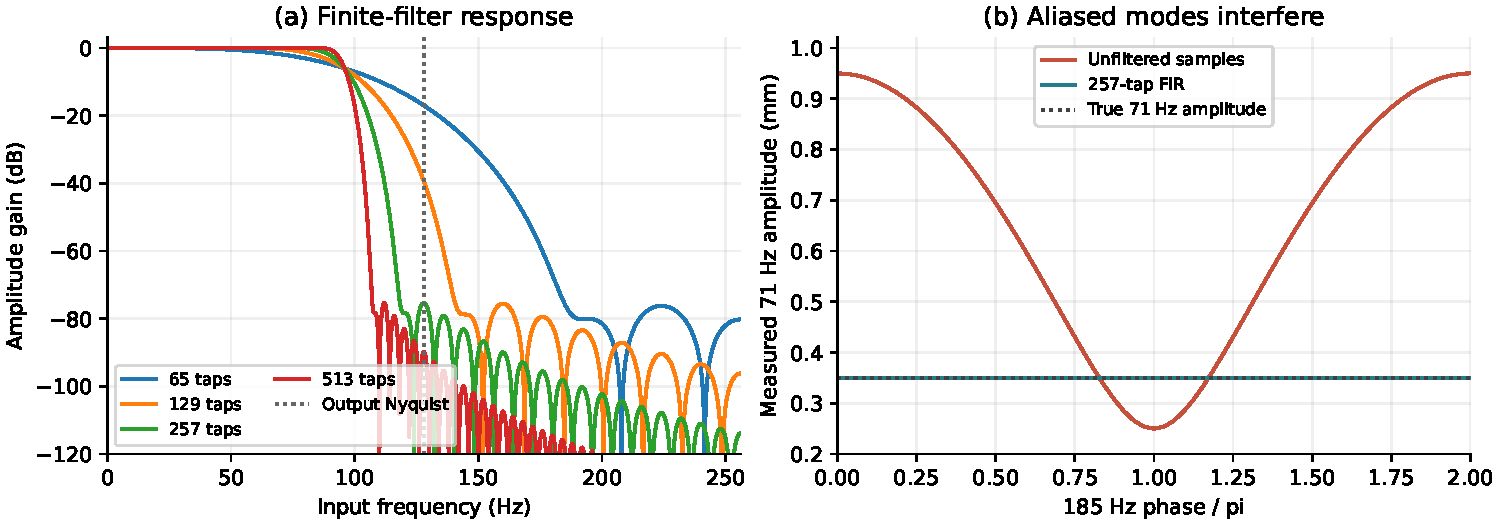
\includegraphics[width=\linewidth]{../examples/results/alias_budget.pdf}
 \caption{Project-generated frequency responses and measured modal interference.
 The finite-filter transition affects the desired 71 Hz mode. The phase sweep
 reveals an amplitude ambiguity after unfiltered sampling; the 257-tap output
 stays close to the prescribed desired amplitude.}
 \label{fig:study}
\end{figure}

Run \texttt{aliasguard --output examples/reproduced} after installing the package.
The committed JSON and three CSV files contain the setup, all filter and phase
results, and the full time record. The paper's numerical macros are generated
from that JSON; input and PDF hashes bind the manuscript to the source and data.

\newpage
\section{Measured results and independent verification}
Table~\ref{tab:results} reports the zero-phase case. Low-band RMSE compares with
$x_{\mathrm{low}}(t)=\cos(2\pi23t)+0.35\cos(2\pi71t)$ mm, not with the full
three-mode signal. Without filtering, this RMSE is \RawRMSE\ mm. A 65-tap
filter nearly removes the high mode but loses substantial desired-mode amplitude.
At 257 taps, the residual-alias bound is $\FineAlias$ mm while the passband
bound is $\FineBias$ mm; the latter is larger. Over all sampled phases,
the measured amplitude lies between \FilteredMin\ and \FilteredMax\ mm.

\begin{table}[h!]
\centering\small
\caption{Measured filter-length study. Signed $g(185)$ is retained because its
sign changes the interference. RMSE is relative to the prescribed low-band signal.}
\label{tab:results}
\begin{tabular}{@{}rrrrrr@{}}
\toprule
$L$ & Delay (ms) & $g(71)$ & $g(185)$ & Amplitude (mm) & RMSE (mm)\\
\midrule
\FilterRows
\bottomrule
\end{tabular}
\end{table}

Independent SciPy implementations~\cite{scipy} verify causal convolution,
Blackman-windowed design and frequency response. Across the four filters, maximum
differences are $\ConvError$ mm, $\DesignError$ in coefficients, and
$\ResponseError$ in complex response. An analytical harmonic prediction using
the centered transfer gains agrees with the retained time samples within
$\HarmonicError$ mm. The independent phasor expression in Eq.~\eqref{eq:bound}
agrees with measured amplitudes over the phase sweep within $\PhaseError$ mm.
These local values are recorded outputs, not universal roundoff bounds.

Tests additionally verify phase reversal, startup, reset, chunk invariance,
DC preservation, malformed inputs and the amplitude bound. Reproduction permits
relative tolerance $2\times10^{-7}$ and absolute tolerance $5\times10^{-12}$ in
each stored field's units across compilers/libraries. CI tests native and Python
builds and installed wheels on Windows and Ubuntu; Linux also checks address and
undefined-behavior sanitizers. Its independent pdfLaTeX manuscript build enforces
at most five pages, resolves citations and rejects overfull boxes. Rendered pages
are inspected separately from automated numerical checks.

\section{Discussion, limitations and conclusion}
Three distinctions matter. First, differences against convolution and phasor
references measure \emph{discrete implementation error}. Second, low-band RMSE
and amplitude bias measure \emph{processing distortion}; even an exactly
implemented FIR deliberately changes the input. Third, no \emph{continuum error}
or physical-validation claim follows: there is no PDE mesh and the prescribed
modal trajectories are evaluated analytically. An actual structure could contain
unmodeled modes, damping and nonlinearities. Sensor noise, ADC quantization,
uncertain frequencies and prior acquisition aliasing are omitted.

Increasing length does not monotonically decrease gain at a single stopband
frequency: 129 taps happen to reject 185 Hz more strongly than 257 taps, while
preserving 71 Hz less accurately. Choosing a filter therefore requires passband
and stopband criteria together with acceptable latency. A finite FIR cannot
guarantee rejection of every signal beyond output Nyquist. The synthetic coherent
record and known-frequency regression do not assess blind modal identification.

AliasGuard's main result is a reproducible two-part amplitude-error account.
For this model, filtering before decimation largely preserves the desired mode,
whereas downsampling first produces an irreducible ambiguity. The analytical
bound makes the tradeoff between wanted-mode distortion and residual aliasing
explicit; it must be reassessed for other spectra and acquisition chains.

\begin{thebibliography}{9}\small
\bibitem{sampling} S. W. Smith. \emph{The Scientist and Engineer's Guide to Digital
Signal Processing}, Ch.~3, ``The Sampling Theorem.''
\url{https://dspguide.com/ch3/2.htm}.
\bibitem{filter} S. W. Smith. Same work, Ch.~16, ``Designing the Filter.''
\url{https://www.dspguide.com/ch16/2.htm}.
\bibitem{scipy} SciPy developers. Signal processing API: \texttt{firwin},
\texttt{lfilter}, \texttt{freqz}. \url{https://docs.scipy.org/doc/scipy/reference/signal.html}.
\end{thebibliography}
\end{document}
